
\section{Specification \& Design}\label{Specification_design}
\subsection{Agile sprints}
An agile sprint is a short timeframe where dedicated efforts are focused on a small number of goals. They were utilised for several components of the project, with not only a usage in the software engineering side, but also on the project management end. A list of these sprints can be found in the appendix, namely \cref{appendix:sprints_list}.

\subsection{Key engineering requirements}
\subsubsection{Key functional requirements}
The key functional requirements include:
\begin{itemize}
\item \lintexspaced must allow users to upload one \latexspaced file, preview the generated \acrshort{pdf} file, and download it if they request.
\item \lintexspaced must detect and recommend fixes for \gls{tagging} and lack of \gls{alt_text}.
\item \lintexspaced must provide useful error messages, in accordance with objective \ref{intro:objective:errors_useful}.
\end{itemize}
The full list of functional requirements can be found in the appendix, namely \cref{appendix:func_requirements}.

\subsubsection{Key non-functional requirements}
Non-functional requirements include:
\begin{itemize}
\item The website should be reasonably efficient.
\item The website should be flexible with supported browsers and desktop screen sizes.
\item The website should be reasonably accessible.
\item \lintexspaced should have thorough documentation describing its usage and code. This conforms to the objective \ref{intro:objective:lintex_maintainable}
\end{itemize}
The full list of functional requirements can be found in the appendix, namely \cref{appendix:non_func_requirements}

\subsection{\lintexspaced supported accessibility}\label{specification_design:supported_accessibility}
The key \latexspaced accessibility features supported were:
\begin{enumerate}
\item[\textbf{Document tagging}] The document would have tagging applied through its \verb|\DocumentMetadata| command. This command accepts a language (`lang') key to specify the document language; tagging key to enable tagging; tagging setup (`tagging-setup') key to select the type of tagging applied to the \latexspaced document; \acrshort{pdf} standard (`pdfstandard') key to specify the \acrshort{pdf} standard the document should follow; and the \acrshort{pdf} version (`pdfversion') key to specify the version of the \acrshort{pdf}. The \acrshort{pdf} version should be compatible with the \acrshort{pdf} standard. It should be noted that the \acrshort{pdf} standard PDF/UA-2 has inconsistencies in version 2.0, which are predicted to be fixed in version 2.1.
\item[\textbf{Table tagging}] Each table should have its tagging standard applied, with the \verb|\tagpdfsetup| command prefixing the tabular group construct, as defined in \fullref{impl:peg_parsing}, with either `table/tagging=presentation' for tables that are read in reading order, or `table/header-rows={N}', where N is the row the headings, for tables where the heading is prefixed before stating a table cell's contents.
\item[\textbf{\Gls{alt_text}}] \verb|\includegraphics| may include \gls{alt_text} applied through the optional key `alt'.
\item[\textbf{Actual text}] \verb|\includegraphics| may include actual text applied through the optional key `actualtext'. Unlike \gls{alt_text}, which has the purpose of describing the text, actual text is used to repeat text extracts within the image itself. For example, a tongue twister.
\item[\textbf{\Gls{artifact}}] \verb|\includegraphics| may include an artifact, applied through the optional key `artifact' with no value or equal sign (`='). This is used to avoid a graphic's screen reader audio output for when a graphic is purely decorative.
\end{enumerate}
All \verb|\includegraphics| are expected to have \gls{alt_text}, actual text, or \gls{artifact}.

Examples of each of these supported accessibility features can be found in \cref{appendix:accessible_doc}.

\subsection{Design patterns used}
\figureref{figure:build_accessible_document} showcases the design patterns involved in the creation of an accessible document. 

\begin{figure}[h]
    \caption{Building an accessible document}\label{figure:build_accessible_document}
    \centering
    \resizebox{0.7\textwidth}{!}{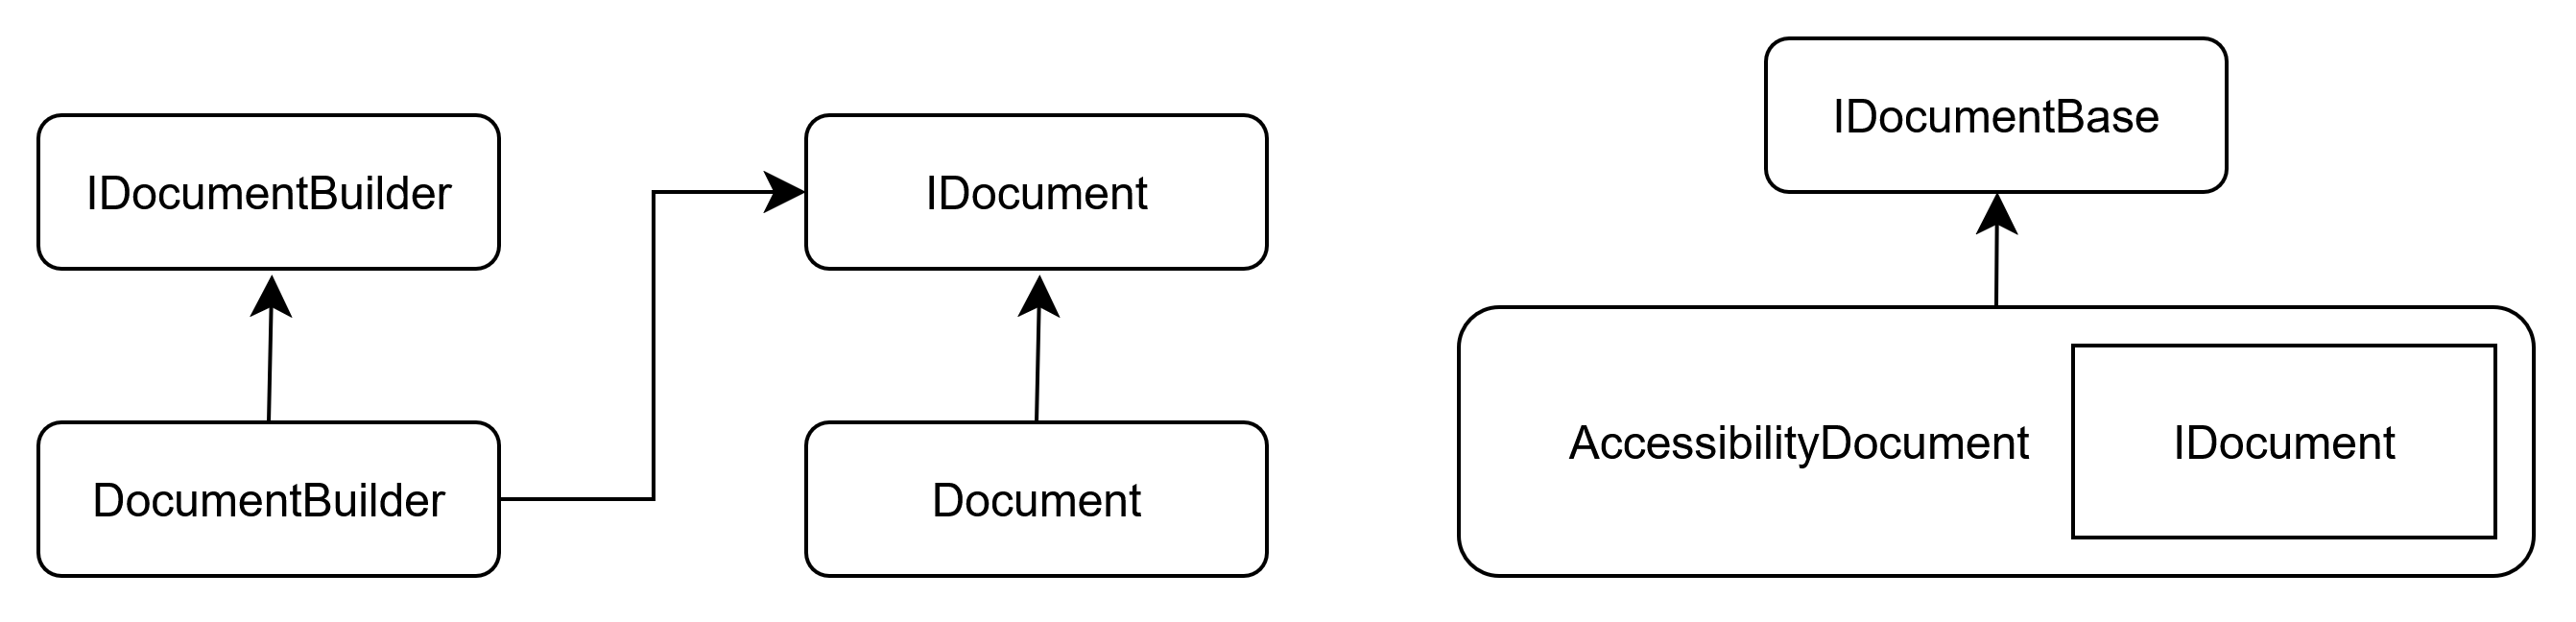
\includegraphics[alt={Figure showcasing the general structure of an accessible document's creation in \lintex}]{images/build_accessible_document.png}}
\end{figure}

The builder design pattern \parencite{builder_design_pattern} was used to create a document that conforms to the `IDocument' interface, rather than a concrete `Document' class. This was necessary to work together with the wrapper design pattern \parencite{wrapper_design_pattern} to ensure a concrete `AccessibleDocument' class could be created, with it containing the original document conforming to the `IDocument' interface. This promoted the reusability of the concrete `Document' for other contexts, which would not have been possible if the builder pattern had created a concrete `AccessibleDocument' from the start.

The Composite design pattern \parencite{composite_design_pattern} was utilised for the handling of the document content, as showcased in \figureref{figure:latex_doc_parsing_structure}. This ensured that both group and line constructs could be treated uniformly through a common interface. 

\fullref{impl:peg_parsing} describes how arguments were written to conform to a common interface, ensuring compliance with the dependency inversion principle \parencite{dependency_inversion}.
\subsection{Error handling}
Below is a diagram showcasing the general structure of error management in \lintex :

\begin{figure}[h]
    \caption{Error handling in \lintex}\label{figure:error_structure}
    \centering
    \resizebox{0.7\textwidth}{!}{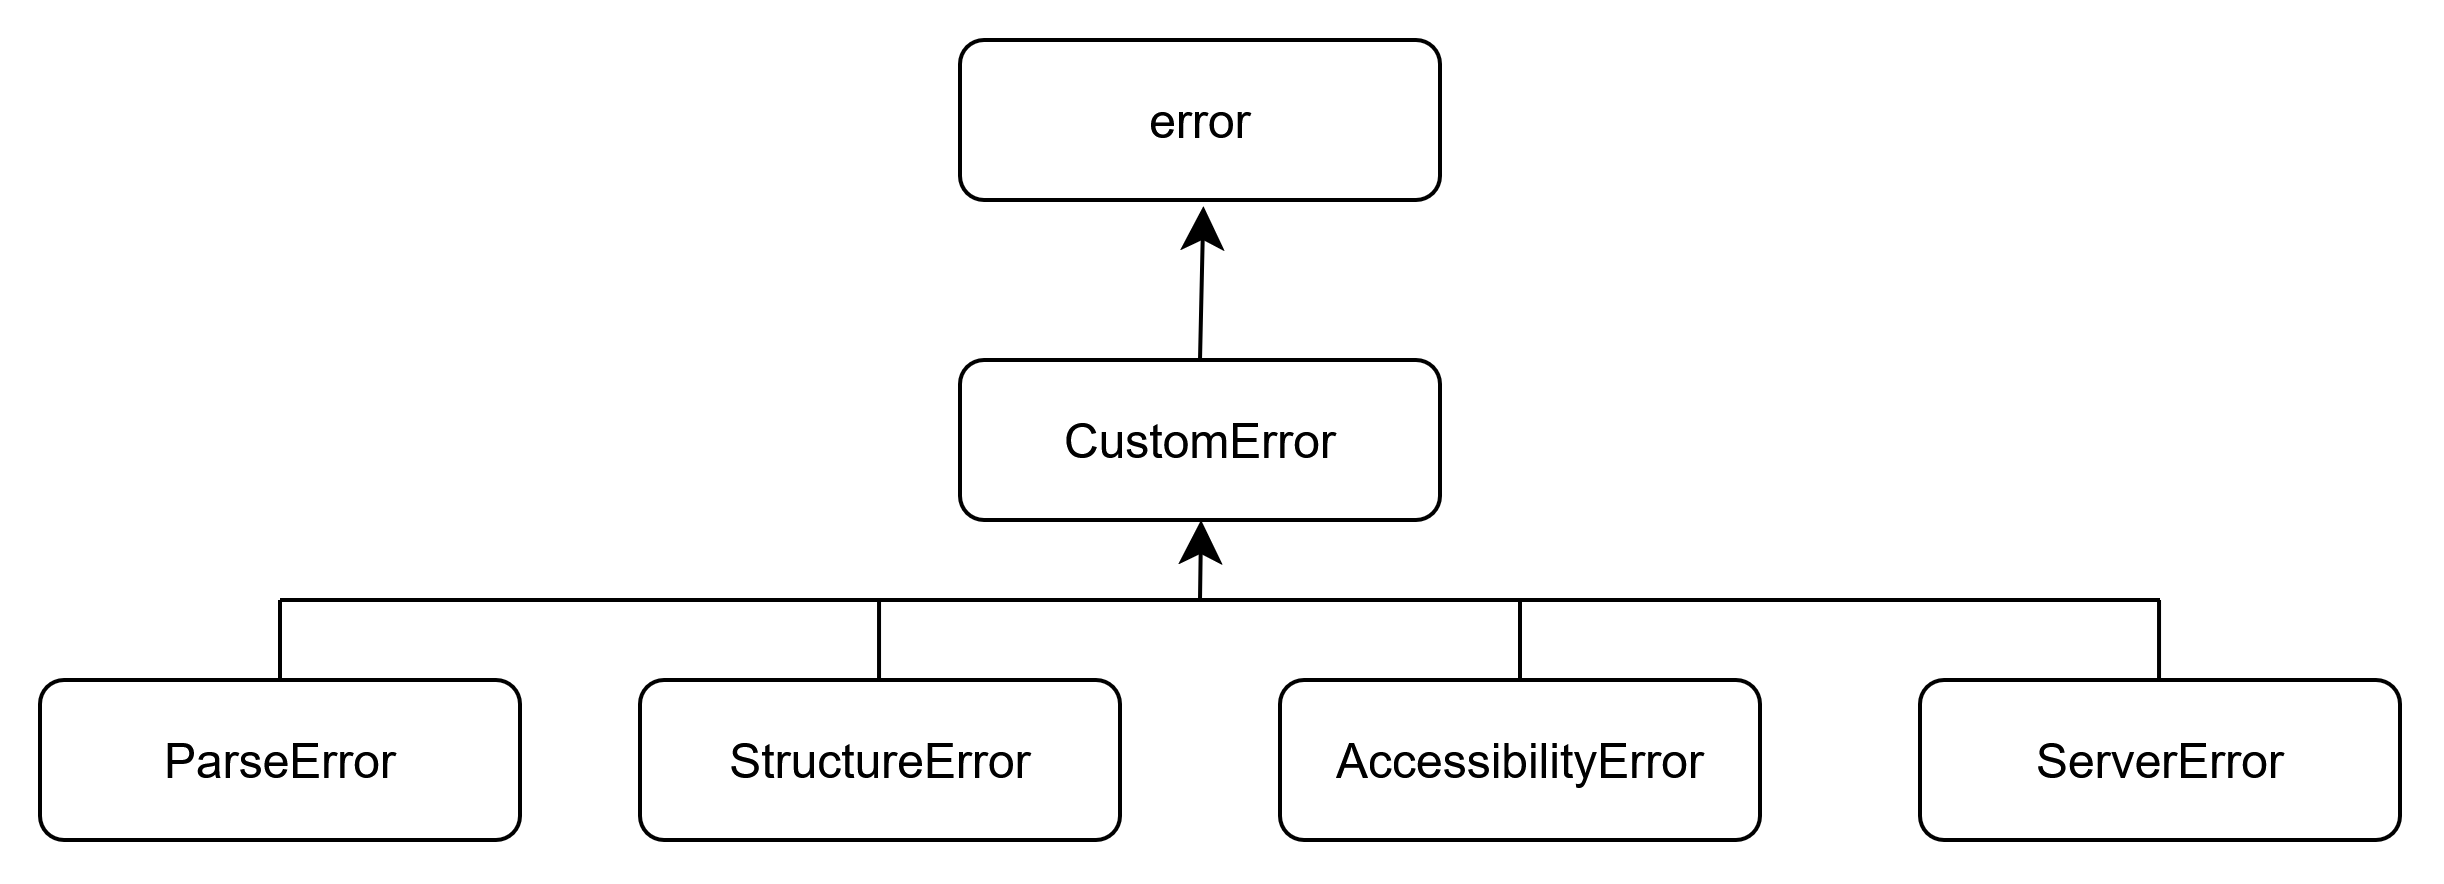
\includegraphics[alt={Figure showcasing the general structure of error handling in LinTex}]{images/error_structure.png}}
\end{figure}

Error handling in \lintexspaced follows the dependency inversion principle \parencite{dependency_inversion}. In Go, all errors are written to the `error' interface. However, it was necessary to create our own interface, `CustomError', to have special handling of data, while still conforming to the `error' interface. From that point, it is relatively simple to have error classes such as `StructureError' conform to the `CustomError' interface.

Another important point is to avoid the repetition of data in an error. For example, the `CustomError' interface implements separate \verb|LongError()| and \verb|Error()| methods. Repeating the description of the \verb|LongError()| in several locations would likely lead to mistakes and additional work in keeping them updated. Hence, a custom function type, `CreateError', was created to compile the error while only necessitating the location information of the error. This worked by creating a helper function that returned the `CreateError' function type, and provided the consistent data between errors to the helper function, such that the `CreateError' function type would only require the location information of the error. The full error list can be found in the appendix in \cref{appendix:err_list}.
\subsection{Documentation}
Thorough documentation has been provided in the form of comments in code, with special emphasis on the \acrshort{peg} script in \cref{appendix:peg_script}. Additionally, the `README.md' contains thorough steps focused on prerequisite installations, installation steps, and steps for contributing to the project.